Automatic abstracting can be done using various techniques in both strong and weak NLP. In this report we focus on three techniques, all using strong NLP. All the techniques discussed rely on some amount of text pre-processing, which involves preparing the text to be in an appropriate format to perform the summarization. Pre-processing of text to prepare for text summarization can be done in fine detail, or can simply involve splitting the text into sentences. The higher the level of detail applied to the pre-processing, the more likely the algorithm will provide valuable results.


\subsection{Nested Tree}
The nested tree automated abstracting technique focuses on finding and classifying inter-sentence and inter-word dependencies. The first step to this algorithm, is to divide the text into sentences, adding a node to the tree for every sentence. The edge connecting the sentence nodes in the tree represents the dependency between the two sentence nodes. This is shown in Figure~\ref{fig:tree}. Nodes connected by edges are adjacent sentences, and the type of dependency between the nodes is what is held in the edge. Words are stored similarly. 

\begin{figure}[H]
	\centering\bf\footnotesize
	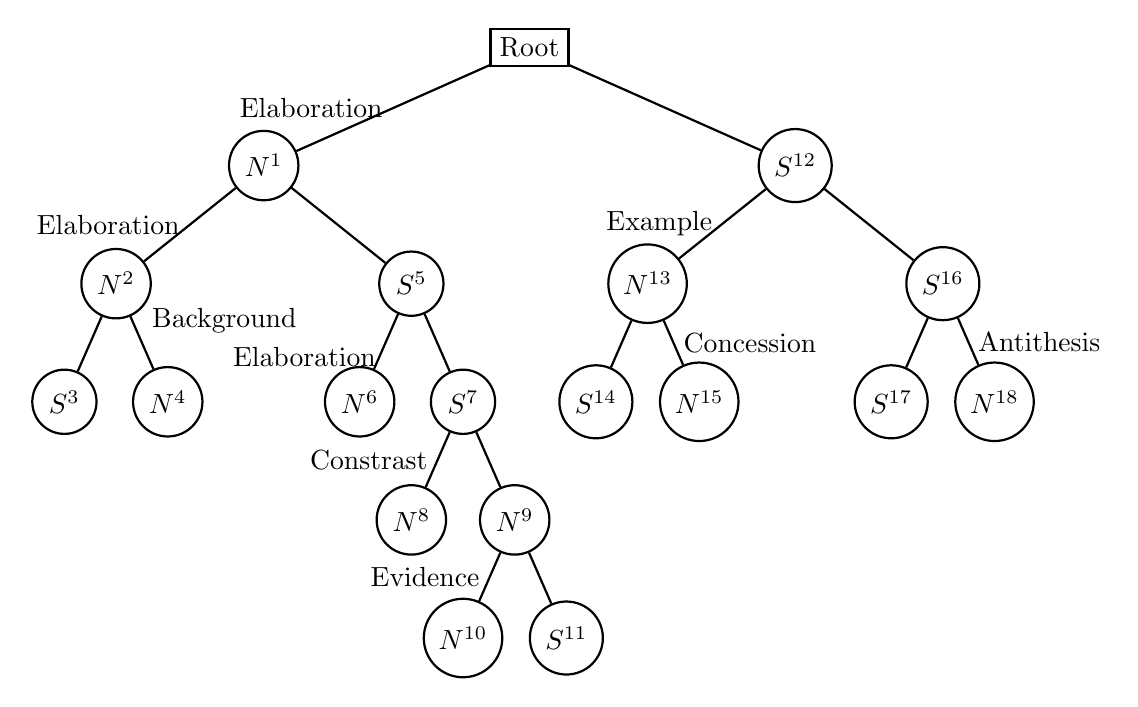
\begin{tikzpicture}[scale=0.75,
	level distance=2cm,
	level 1/.style={sibling distance=9cm},
	level 2/.style={sibling distance=5cm},
	level 3/.style={sibling distance=1.75cm},
	root node/.style={thick, draw},
	tree node/.style={thick, circle,draw},
	every child node/.style={tree node}]
	
	\node[root node] (Root) {Root}
	child[thick] {
		node[tree node] {$N^1$} 
		child { node[tree node] {$N^2$} 
			child { node[tree node] {$S^3$} }
			child { node[tree node] {$N^4$} edge from parent node[right] {\raisebox{1.5pc}{Background}} }
			edge from parent node[left] {Elaboration}
		}
		child { node[tree node] {$S^5$} 
			child { node[tree node] {$N^6$} edge from parent node[left] {\raisebox{-1.5pc}{Elaboration}} } 
			child { node[tree node] {$S^7$} 
				child { node[tree node] {$N^8$} edge from parent node[left] {Constrast} }
				child { node[tree node] {$N^9$} 
					child { node[tree node] {$N^{10}$} edge from parent node[left] {Evidence} }
					child { node[tree node] {$S^{11}$} }
				}
			}
		}
		edge from parent node[left] {Elaboration}
	}
	child[thick] {
		node[tree node] {$S^{12}$}
		child { node[tree node] {$N^{13}$} 
			child { node[tree node] {$S^{14}$} }
			child { node[tree node] {$N^{15}$} edge from parent node[right] {Concession} }
			edge from parent node[left] {Example}
		}
		child { node[tree node] {$S^{16}$}
			child { node[tree node] {$S^{17}$} }
			child { node[tree node] {$N^{18}$} edge from parent node[right] {Antithesis}}	
		}
	};
	\end{tikzpicture}
	\caption{Conceptual Diagram of the Nested Tree Approach\label{fig:tree}}
\end{figure}

Each sentence is split into words which are each stored in a word node. These nodes are each stored in a tree within each sentence node. In each word tree, the dependency between the words is held in the edge between the two dependent word nodes. 
Therefore when conceptualizing the tree, it is important to note that the dependency between word nodes forms the meaning and the dependency between sentence nodes essentially determines the meaning of the entire sentence. 
When forming edges, there are many different types of dependencies, each of which can be classified as either a core sentence attribute, or a dependency attribute which adds additional meaning or value to a core sentence. To form the summary, we start from the lowest branches in the tree, and we begin trimming. When performing the tree trimming to obtain our summary, we first trim the sentences whose dependency trees indicate that they add little value to the text as a whole. Core dependencies are the sentence nodes to be trimmed last as they are the core meaning of the sentence and are therefore an important sentence to the summary. This method will form a concise summary by continuously trimming the tree until we reach the desired summary length. It's important to note that this summary method allows us to trim the summary to any length we chose. The disadvantage of this, is that very short summaries may be concise but are likely to also lack information that is important to the meaning of the sentence, resulting in an incomplete and therefore inaccurate summary of the text. 

\subsection{Evolutionary Algorithm}
The evolutionary algorithm approach to automated abstraction is a more complicated approach in comparison to the nested tree method. This method also requires more time and computational power.

Initially, a {\em population} of candidate summaries are created from the original text. This population is essentially just a multiset containing not necessarily distinct subsets of set of sentences from the original text. \edit{Wordy?} Then, each candidate summary is scored.

Some possible scoring parameters are the sentence's position in a paragraph (the first sentence in a paragraph being awarded one point, the second $4 \over 5$, the third $3\over 5$, and so on), font style such as capitalized or bold-face type, or the presence of numerical or temporal information in the sentence. Each of these scoring parameters which identify favourable text features would add to a sentence's overall score. Hence sentences with higher scores are regarded as being more significant to the text's meaning.

Following this scoring --- known as {\em fitness evaluation} in the genetic algorithm field --- candidate summaries are chosen to become parents and produce offspring. Like reproduction in nature, reproduction in an evolutionary algorithm relies on crossover and mutation operators. An example of crossover to maximize child fitness is the case where two candidate summaries $S_1$ and $S_2$ each contain a very fit sentence (the fit sentence in $S_1$ not equal to the sentence in $S_2$).


\subsection{Graphs}
Graph based automated abstraction techniques are similar to the tree method. First the text to summarize is broken down into individual sentences. These sentences are then placed into nodes which are initially connected by edges representing the adjacency of sentences in the text. Once all the nodes have been added to the tree. The missing edges representing other criteria within the sentence are added, these criteria can range from the type of sentence, to shared or similar words. When all the edges have been added to the graph, the graph is now considered full. To get the summary of the text from the graph, we must simply determine the sentences with the most dependencies (largest number of edges connected to the node). The number of sentence to be chosen to create the summary will dictate the length of the summary. While the graph based method can give accurate detailed summaries, they are extractive, in that they will not add anything additional to the text to form the summary, but will instead simply extract the important elements in the text and add them to the summary. In the case of applying this using the graph based approach, results in a severly fragmented summary, resulting from simply printing out the summary sentences in bullet point form. While this technique has good results, in would not be capable of creating a paragraph summary which is smooth to read and grammatically correct.
